\documentclass{beamer}
\usetheme{Warsaw}

\setbeamercolor{normal text}{fg=white,bg=black!90}
\setbeamercolor{structure}{fg=white}

\setbeamercolor{alerted text}{fg=red!85!black}

\setbeamercolor{item projected}{use=item,fg=black,bg=item.fg!35}

\setbeamercolor*{palette primary}{use=structure,fg=structure.fg}
\setbeamercolor*{palette secondary}{use=structure,fg=structure.fg!95!black}
\setbeamercolor*{palette tertiary}{use=structure,fg=structure.fg!90!black}
\setbeamercolor*{palette quaternary}{use=structure,fg=structure.fg!95!black,bg=black!80}

\setbeamercolor*{framesubtitle}{fg=white}

\setbeamercolor*{block title}{parent=structure,bg=black!60}
\setbeamercolor*{block body}{fg=black,bg=black!10}
\setbeamercolor*{block title alerted}{parent=alerted text,bg=black!15}
\setbeamercolor*{block title example}{parent=example text,bg=black!15}

\setbeamertemplate{headline}{}

\usepackage[brazil,spanish]{babel}
\usepackage[utf8]{inputenc}
\documentclass[11pt]{article}
\usepackage{color}
\usepackage{listings}
\usepackage{setspace}
\usepackage{minted}
\usepackage[demo]{graphicx}
\usepackage{changepage}

%GiacoStuff
\usepackage{ulem}
\usepackage{etoolbox,refcount}
\usepackage{multicol}

\newcounter{countitems}
\newcounter{nextitemizecount}
\newcommand{\setupcountitems}{%
  \stepcounter{nextitemizecount}%
  \setcounter{countitems}{0}%
  \preto\item{\stepcounter{countitems}}%
}
\makeatletter
\newcommand{\computecountitems}{%
  \edef\@currentlabel{\number\c@countitems}%
  \label{countitems@\number\numexpr\value{nextitemizecount}-1\relax}%
}
\newcommand{\nextitemizecount}{%
  \getrefnumber{countitems@\number\c@nextitemizecount}%
}
\newcommand{\previtemizecount}{%
  \getrefnumber{countitems@\number\numexpr\value{nextitemizecount}-1\relax}%
}
\makeatother    
\newenvironment{AutoMultiColItemize}{%
\ifnumcomp{\nextitemizecount}{>}{3}{\begin{multicols}{2}}{}%
\setupcountitems\begin{itemize}}%
{\end{itemize}%
\unskip\computecountitems\ifnumcomp{\previtemizecount}{>}{3}{\end{multicols}}{}}
%GiacoStuffn't

\linespread{1.15} \\
%%%%%%%%%%%%%%%%%%%%%%%%%%%%%%%%%%%%%%%%%%%%%%%%



\title[Proyecto de Memoria - MAT301]{Análisis Estadístico de Imágenes usando la transformación de Box y Cox}
% Titre du diaporama

% Sous-titre optionnel

\author{Fabián Castellano Núñez}
% La commande \inst{...} Permet d'afficher l' affiliation de l'intervenant.
% Si il y a plusieurs intervenants: Marcel Dupont\inst{1}, Roger Durand\inst{2}
% Il suffit alors d'ajouter un autre institut sur le modèle ci-dessous.

\institute[Universidad Técnica Federico Santa María]
  {
  Profesor Guia: Ronny Vallejos
  }


\date{26 de Julio,  2022}
% Optionnel. La date, généralement celle du jour de la conférence

\subject{Transformación BoxCox}
% C'est utilisé dans les métadonnes du PDF
\titlegraphic{
    
\includegraphics[width=3cm,keepaspectratio]{logo_dmat.png}%
    \hfill%
    
\includegraphics[width=2cm,keepaspectratio]{logo_usm3.png}%
}
%%%%%%%%%%%%%%%%%%%%%%%%%%%%%%%%%%%%%%%%%%%%%%%%%%%%%%%%%%%%%%%%%%%%%
\begin{document}

\begin{frame}
  \titlepage
\end{frame}

\begin{frame}{Contenidos}
  \tableofcontents
  % possibilité d'ajouter l'option [pausesections]
\end{frame}




\section{La transformación BoxCox}

\begin{frame}{La transformación BoxCox}
    \pause
    \begin{block}{Transformación BoxCox}
    Como fue definida por Box y Cox en 1964 \cite{boxcox}
        \begin{equation}\label{boxcox}
            y^{(\lambda)}= \begin{cases}\frac{y^{\lambda}-1}{\lambda} & (\lambda \neq 0) \\ \log y & (\lambda=0)\end{cases}
        \end{equation}
    \end{block}
        \pause
    \begin{block}{Verosimilitud}
        \begin{equation*}
            \mathcal{L}(\lambda) \equiv-\frac{n}{2} \log \left[\frac{1}{n} \sum_{j=1}^{n}\left(x_{j}^{\lambda}-\overline{x^{\lambda}}\right)^{2}\right] +(\lambda-1) \sum_{j=1}^{n} \log x_{j}
        \end{equation*}
    \end{block}
    
\end{frame}
\section{BoxCox sobre imágenes}
\begin{frame}{La transformación BoxCox sobre imágenes}
    \pause
    \begin{block}{Transformación 1-D}
        Transformar la imagen a un vector unidimensional, usar estos datos para determinar $\lambda$.
    \end{block}
    
        \pause
        
    \begin{block}{Histograma}
        La idea es usar el histograma como un proxy comprimido de de la matriz de datos. 
    \end{block}
        \pause
    
    La correlación entre estos dos números encontrada de forma experimental fue $r^2=-0.3022$ (Cheddad, 2020) \cite{cheddad2020}. La diferencia de tiempo de calculo entre las dos versiones es de 2 ordenes de magnitud
    -
\end{frame}

\begin{frame}{Ejemplos}
\begin{figure}
    \centering
    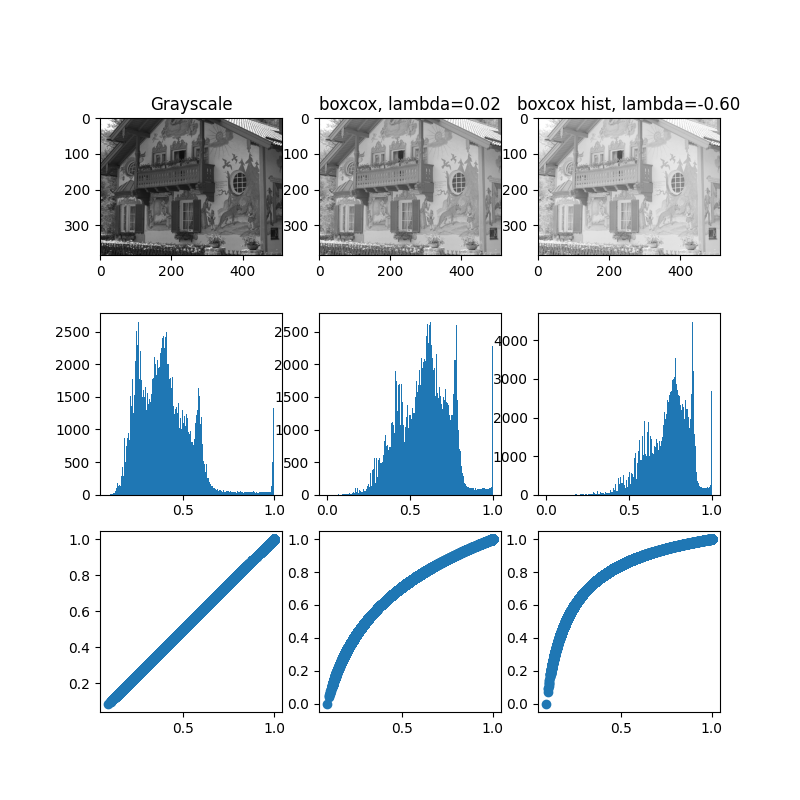
\includegraphics[scale=0.3] {plot_I24.BMP.png  }
    \label{fig:my_label}
\end{figure}

\end{frame}
\begin{frame}{Ejemplos}
\begin{figure}
    \centering
    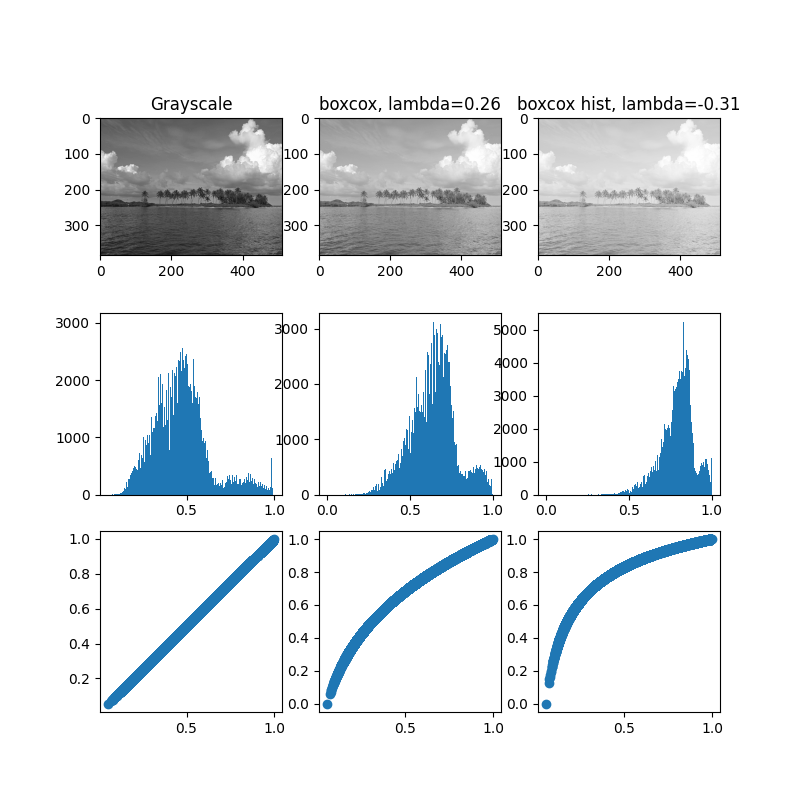
\includegraphics[scale=0.3] {plot_I16.BMP.png  }
    \label{fig:my_label}
\end{figure}

\end{frame}
\begin{frame}{Ejemplos}
\begin{figure}
    \centering
    \includegraphics[scale=0.3] {plot_I25.BMP.png  }
    \label{fig:my_label}
\end{figure}

\end{frame}

\section{Estado del arte}
\begin{frame}{Estado del arte}
    \pause
    \begin{block}{On Box-Cox Transformation for Image Normality and Pattern Classification (Cheddad, 2020) \cite{cheddad2020}}
        \begin{figure}
            \centering
            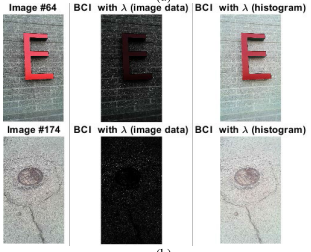
\includegraphics[scale=0.7] {paperbcim2.png}
            \label{fig:my_label}
        \end{figure}
    \end{block}    
\end{frame}
\begin{frame}{Estado del arte}
    \begin{block}{On Box-Cox Transformation for Image Normality and Pattern Classification (Cheddad, 2020) \cite{cheddad2020}}
        \begin{figure}
            \centering
            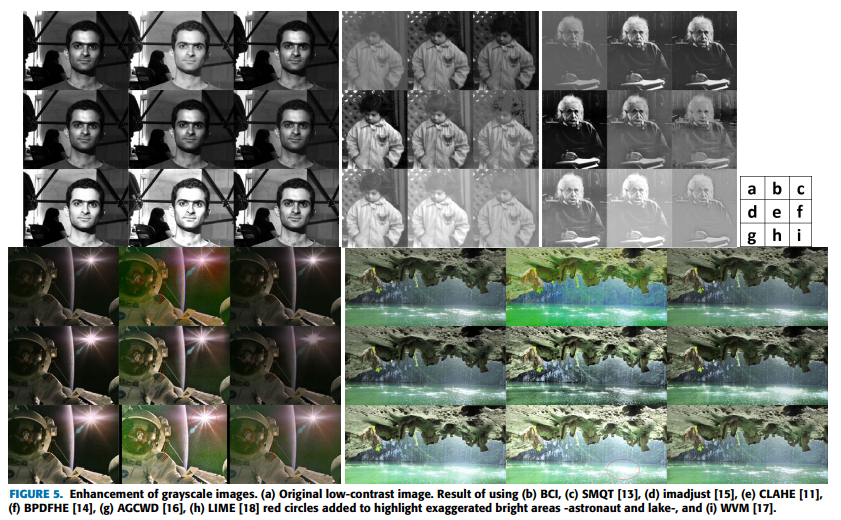
\includegraphics[scale=0.4] {paperbcim1.png}
            \label{fig:my_label}
        \end{figure}
    \end{block}    
\end{frame}
\begin{frame}{Estado del arte}
    \pause
        \begin{block}{MR Image Segmentation Using a Power Transformation Approach (Juin-Der Lee et al., 2009) \cite{juin2009} }
        \begin{figure}
            \centering
            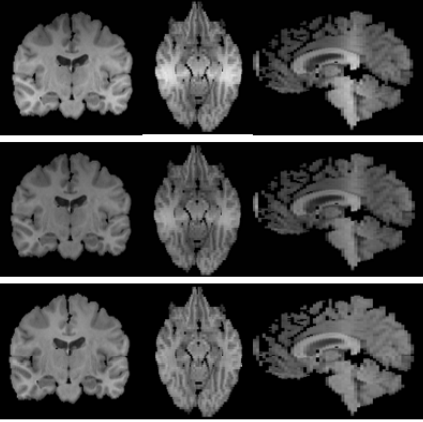
\includegraphics[scale=0.6]{papermri1.png}
            \label{fig:my_label}
        \end{figure}
    \end{block}
\end{frame}


\section{Metodología: Comparación entre imágenes}
\subsection{Coeficiente de Información Máxima}

\begin{frame}{Metodología: Coeficiente de Información Máxima}
    \pause
    
    \begin{block}{Información mutua}
    Dada una distribución bivariada $P(x,y)$, definimos:
        \begin{equation}\label{información mutua}
            \mathrm{I}(X ; Y)=\int_{\mathcal{Y}} \int_{\mathcal{X}} P_{(X, Y)}(x, y) \log \left(\frac{P_{(X, Y)}(x, y)}{P_{X}(x) P_{Y}(y)}\right)dxdy
        \end{equation}
    \end{block}
    \pause


    \begin{block}{Máximo sobre todas las mallas}
        Para un conjunto finito $D\in\mathcal{R}  ^2$ y enteros positivos $x,y$, definimos:
		$$
		I^*(D,x,y)=\max I(D|_G)
		$$
    \end{block}
    \begin{figure}
        \centering
        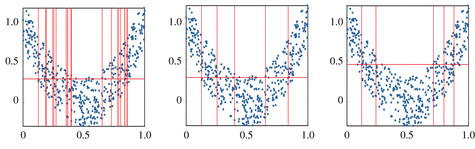
\includegraphics[scale=0.6] {rsos201424f03.png}
        \label{fig:my_label}
    \end{figure}
\end{frame}

\begin{frame}{Metodología: Coeficiente de Información Máxima}
    \begin{block}{Matriz Característica}
        Definimos la siguiente matriz       
        \begin{equation}
	    	M(D)_{x, y}=\frac{I^{*}(D, x, y)}{\log \min \{x, y\}}
        \end{equation}
        Notemos que en principio la matriz es infinita.
    \end{block}
    \pause

    \begin{block}{Coeficiente de Información Máxima}
        Definido en por Reshef en 2011 \cite{reshef2011} Dado un conjunto de datos bivariado, tenemos:
        \begin{equation}\label{MIC}
	    	\operatorname{MIC}(D)=\max _{x y<B(n)}\left\{M(D)_{x, y}\right\}
        \end{equation}
        donde $\omega(1)<B(n) \leq O\left(n^{1-\varepsilon}\right)$ para alg\'un $0<\varepsilon<1$. En el artiuclo utilizan $B(n)=n^{0.6}$
    \end{block}
\end{frame}

\subsection{Correlaci\'on local}

\begin{frame}{Metodología: Correlaci\'on local}
    \pause
    \begin{block}{Integral de correlación}
        Dada una serie de tiempo $\{z_i\}_{i=0}^{N}$, se define:
        \begin{equation}\label{información mutua}
            I(r)=\lim _{N \rightarrow \infty}\left\{\frac{1}{N^{2}} \sum_{i, j=1}^{N} I\left(\left|z_{i}-z_{j}\right|<r\right)\right\}
		\end{equation}
    \end{block}
    \pause
	Esta integral se puede realizar en datos bivariados, para esto definimos:
    \pause
    \begin{block}{Integral de correlación}
        Dada un conjunto de datos bivariados $\{z_i\}_{i=0}^{N}=\{(x_i,y_i)\}_{i=0}^{N}$, se define:
        \begin{equation}\label{información mutua}
            \hat{I}(r)=\frac{1}{N^{2}} \sum_{i, j=1}^{N} I\left(\left|z_{i}-z_{j}\right|<r\right)
		\end{equation}
    \end{block}
    \end{frame}

    \begin{frame}{Metodología: Correlaci\'on local}
    \begin{block}{Densidad local}
        Calculamos la densidad local como como la derivada de $\hat{I}$
        \begin{equation}
	    	\hat{D}(r)= \frac{\vartriangle\hat{I}(r)}{\vartriangle r}
        \end{equation}
    \end{block}
    \pause
    
   
    
    \begin{block}{Correlación local}
        Sea $\hat{D}_0(r)$ un estimado para una distribución nula, definimos:
        \begin{equation}\label{MIC}
	    	\ell(r)=\widehat{D}(r)-\widehat{D}_{0}(r)
        \end{equation}
    \end{block}
    \pause
    
    \begin{block}{Máxima Correlación Local }
        Como fue definido por  Chen en 2010 \cite{chen2010}, tenemos:
        \begin{equation}\label{MIC}
	    	M=\max _{r}\{|\ell(r)|\}
        \end{equation}
    \end{block}
\end{frame}


\section{Objetivos de la memoria}
\begin{frame}{Objetivos de la memoria}
    \begin{block}{Objetivo Principal}
        Estudiar la efectividad de la transformación de Box y Cox en matrices que poseen información espacial, en particular imágenes, para la resolución de problemas de inferencia y de clasificación.
    \end{block}
    \pause
    \begin{block}{Objetivos Secundarios}
        \begin{itemize}
            \item Estudiar la relación entre una imagen y su transformada de BoxCox
            \item Estudiar la relación entre imágenes antes y después de aplicar la transformación
            \item Generar una versión de la transformación y de los coeficiente que mantenga la información espacial de la imagen
        \end{itemize}
    \end{block}
\end{frame}




\begin{frame}{Bibliografía}
    \begin{thebibliography}{9}
    \bibitem{boxcox}
    Box, G. and Cox, D., 1964. An Analysis of Transformations. Journal of the Royal Statistical Society, 26(2), pp.211-252.
    
    \bibitem{chen2010}
    Chen, Y., Almeida, J., Richards, A., Müller, P., Carroll, R. and Rohrer, B., 2010. A Nonparametric Approach to Detect Nonlinear Correlation in Gene Expression. Journal of Computational and Graphical Statistics, 19(3), pp.552-568.
    
    \bibitem[]{reshef2011}
    Reshef, D., Reshef, Y., Finucane, H., Grossman, S., McVean, G., Turnbaugh, P., Lander, E., Mitzenmacher, M. and Sabeti, P., 2011. Detecting Novel Associations in Large Data Sets. Science, 334(6062), pp.1518-1524.
    
    \end{thebibliography}
\end{frame}

\begin{frame}{Bibliografía}
    \begin{thebibliography}{9}
    \bibitem[]{cheddad2020}
    Cheddad, A., 2020. On Box-Cox Transformation for Image Normality and Pattern Classification. IEEE Access, 8, pp.154975-154983.
    
    \bibitem[]{juin2009}
    Juin-Der Lee, Hong-Ren Su, Cheng, P., Liou, M., Aston, J., Tsai, A. and Cheng-Yu Chen, 2009. MR Image Segmentation Using a Power Transformation Approach. IEEE Transactions on Medical Imaging, 28(6), pp.894-905.
    
    \end{thebibliography}
\end{frame}
\end{document}




